\documentclass[border=10pt]{standalone}

\usepackage{tikz}
\usepackage{tikzsymbols}
\usetikzlibrary{calc,patterns,shapes.geometric}

\def\centerarc[#1](#2)(#3:#4:#5){\draw[#1] ($(#2)+({#5*cos(#3)},{#5*sin(#3)})$) arc (#3:#4:#5);}

\begin{document}
	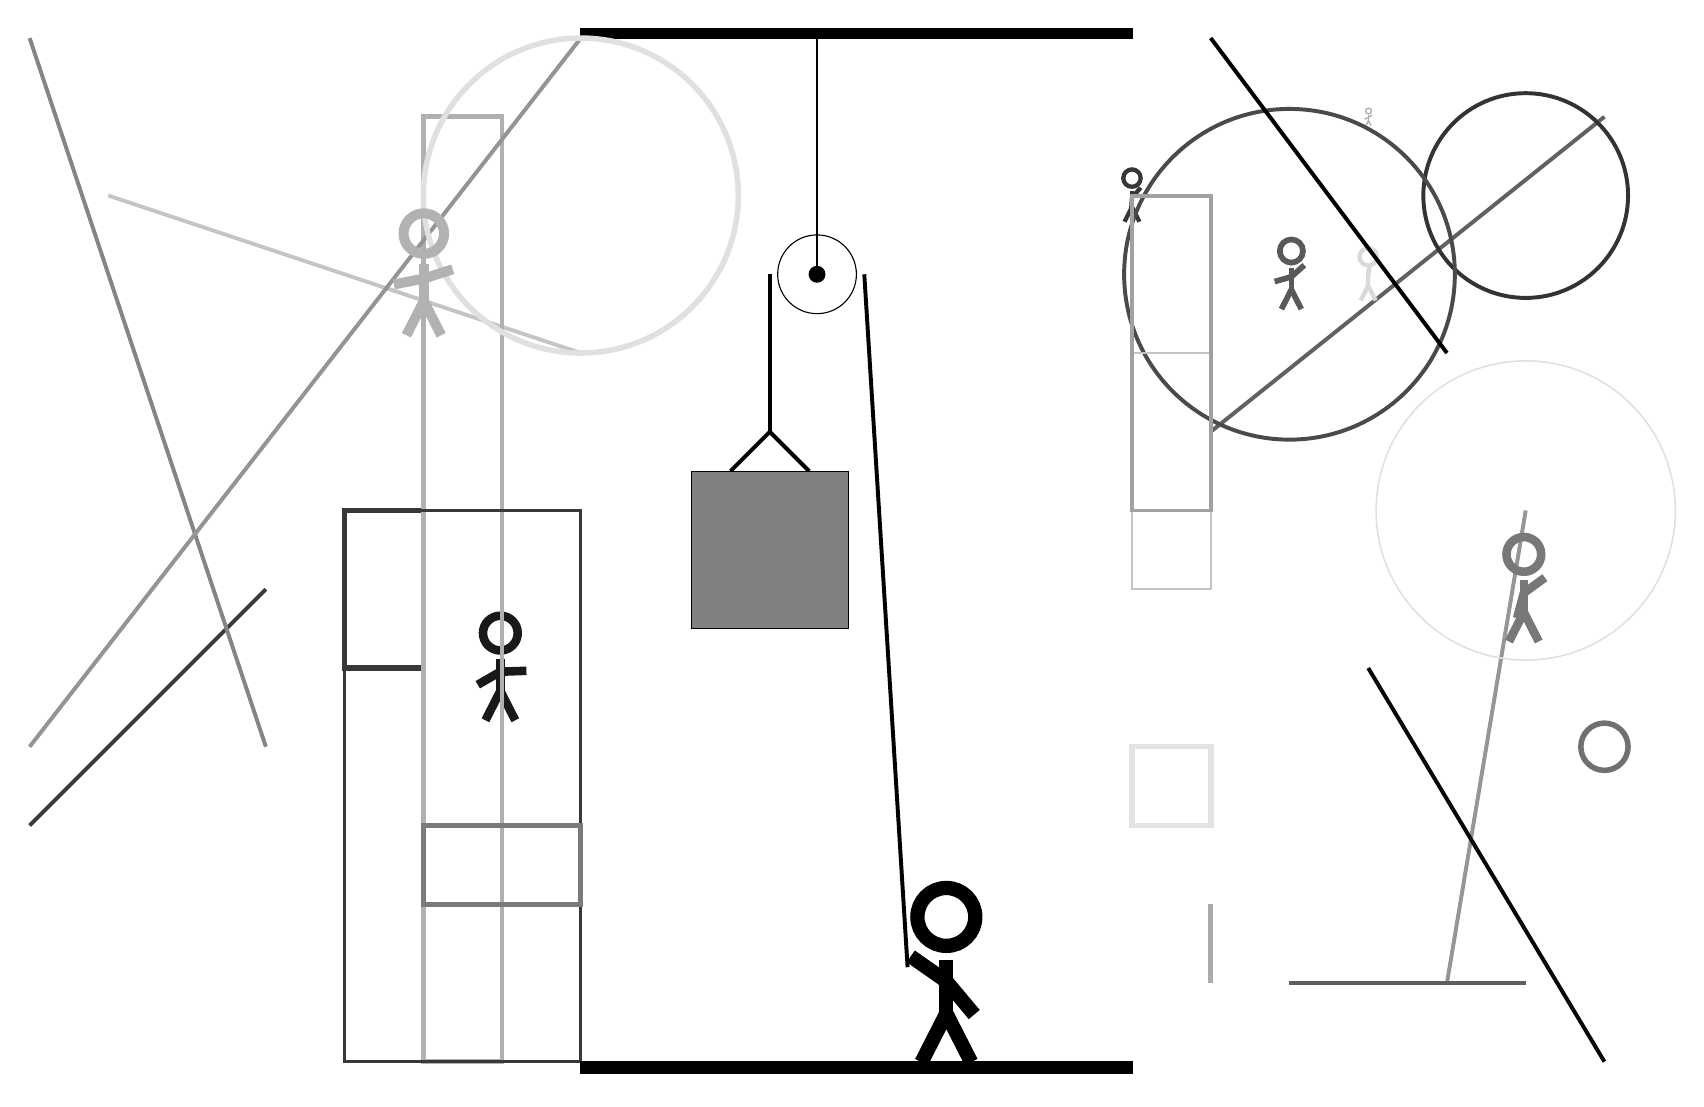
\begin{tikzpicture}
		%%%%% START %%%%%
		
		\draw[fill=black] (-2, 10) rectangle (5, 10.125);
		
		\draw (1, 7) circle (0.5);
		\draw[fill=black] (1, 7) circle (0.1);
		\draw (1, 10) -- (1, 7);
		
		\draw[line width=0.5mm] (-0.1, 4.5) -- (0.4, 5.0) -- (0.9, 4.5);
		\draw[fill=black!50] (-0.6, 4.5) rectangle (1.4, 2.5);
		
		\draw[line width=0.5mm] (0.4, 7) -- (0.4, 5.0);
		\centerarc[line width=0.5mm](1, 7)(0:180:0.6);
		\draw[line width=0.5mm](1.6, 7) -- (2.15, -1.8);
		
		\draw[line width=0.5mm, color=black!62](6, 5) -- (11, 9);
		
		\draw [line width=0.7mm, color=black!56](11, 1) circle (0.3);
		\draw[line width=0.5mm, color=black!23](-2, 6) -- (-8, 8);
		\node[line width=0.7mm, color=black!90] at (-3, 2) {\Strichmaxerl[6][30][2]};
		\node[line width=0.5mm, color=black!31] at (8, 9) {\Strichmaxerl[1][24][37]};
		
		\draw [line width=0.5mm, color=black!80](10, 8) circle (1.3);
		\draw[line width=0.5mm, color=black!41](10, 4) -- (9, -2);
		
		\draw[line width=0.5mm, color=black!97](8, 2) -- (11, -3);
		\draw [line width=0.2mm, color=black!12](10, 4) circle (1.9);
		\draw[line width=0.6mm, color=black!33] (6, -2) rectangle (6, -1);
		
		\draw[line width=0.7mm, color=black!78] (-4, 4) rectangle (-5, 2);
		
		\node[line width=0.3mm, color=black!79] at (5, 8) {\Strichmaxerl[3][86][48]};
		\draw [line width=0.5mm, color=black!71](7, 7) circle (2.1);
		\draw[line width=0.3mm, color=black!23] (6, 6) rectangle (5, 3);
		\draw[line width=0.5mm, color=black!77](-6, 3) -- (-9, 0);
		\draw[line width=0.6mm, color=black!31] (-3, 9) rectangle (-4, -3);
		\node[line width=0.7mm, color=black!65] at (7, 7) {\Strichmaxerl[4][16][42]};
		\node[line width=0.4mm, color=black!15] at (8, 7) {\Strichmaxerl[3][88][84]};
		\draw[line width=0.5mm, color=black!37] (5, 8) rectangle (6, 4);
		\draw[line width=0.5mm, color=black!63](10, -2) -- (7, -2);
		\draw[line width=0.5mm, color=black!48](-6, 1) -- (-9, 10);
		
		\draw[line width=0.5mm, color=black!42](-2, 10) -- (-9, 1);
		
		\draw [line width=0.7mm, color=black!12](-2, 8) circle (2.0);
		\draw[line width=0.7mm, color=black!11] (5, 1) rectangle (6, 0);
		\node[line width=0.3mm, color=black!53] at (10, 3) {\Strichmaxerl[6][75][36]};
		
		\node[line width=0.4mm, color=black!30] at (-4, 7) {\Strichmaxerl[7][11][18]};
		
		\draw[line width=0.4mm, color=black!78] (-2, -3) rectangle (-5, 4);
		\draw[line width=0.5mm, color=black!100](9, 6) -- (6, 10);
		\draw[line width=0.6mm, color=black!52] (-2, 0) rectangle (-4, -1);
		
		\node at (2.6, -1.9) {\Strichmaxerl[10][-35][-50]};
		
		\draw[fill=black] (-2, -3) rectangle (5, -3.15);
		
		%%%%% END %%%%%
	\end{tikzpicture}
\end{document}